\documentclass[11pt,letterpaper]{article}
\usepackage[lmargin=1in,rmargin=1in,bmargin=1in,tmargin=1in]{geometry}
\usepackage{checkins}


% -------------------
% Content
% -------------------
\begin{document}
\thispagestyle{title}

% 08/22
\checkin{08/22} Let $f(x)$ be a relation with $f(2)= 7$ and $f(-3)= 7$. Because $f(2)$ and $f(-3)$ are both $7$, $f$ cannot be a function. \pspace

\sol The statement is \textit{false}. A relation is a function if there is only one possible output for a given input, i.e. given an input, one knows with certainty what the output is. We know that $f(2)= 7$ and $f(-3)= 7$; that is, given the inputs of $x= 2$ or $x= -3$, we know the output. The fact that the outputs are the same is irrelevant. There are many functions with the property that $f(2)= 7$ and $f(-3)= 7$. For instance, there must be a linear function through these two points, i.e. $y= 7$. An example of a quadratic function through these points is $y= \frac{7x(x + 1)}{6}$. \pvspace{1.3cm}



% 08/27
\checkin{08/27} If $S(t)= 0.008t + 57.81$ represents the stock price for a company $t$ minutes after opening, then the rate of change of the stock value is $0.008$, i.e. the stock is gaining $\$0.008$ per minute in value, and the opening price of the stock was $\$57.81$. \pspace

\sol The statement is \textit{false}. The stock price at opening would be the stock price at $t= 0$. But $S(0)= 0.008(0) + 57.81= 57.81$. Therefore, the opening stock price was \$57.81. Observe that $S(t)$ is a linear function, i.e. a function of the form $y= mx + b$ with $y= S$, $x= t$, $m= 0.008$, and $b= 57.81$. We know the rate of change of a linear function is its slope. But then the rate of change of $S(t)$ is $m= 0.008$, i.e. there is an increase of \$0.008 per minute in the value of the stock. \pvspace{1.3cm}



% 08/29
\checkin{08/29} If the production cost of a certain item is constant, then the cost to produce $q$~items, $C(q)$ is linear. Furthermore, the slope of $C(q)$ is the marginal cost and $C(0)$ is the fixed cost. \pspace

\sol The statement is \textit{true}. If the cost of production for the item is constant, then the production cost has a constant rate of change. But then the cost function to produce $q$ items, $C(q)$, must be linear. We know the marginal cost for a linear cost function is its slope. Furthermore, $C(0)$ is the fixed costs. But the $y$-intercept of $C(q)$ is precisely $C(0)$. \pvspace{1.3cm}



% 09/03
\checkin{09/03} Let $f(x)= 17(0.93)^x$. Because $f(x)$ the form $Ab^x$ with $A= 17$ and $b= 0.93$, it is exponential. Furthermore, $A= 17$ represents the $y$-intercept of $17$, i.e. an initial value of $17$, and $b= 0.93$ can be interpreted as a 93\% decrease of the initial value of $17$ a total of $x$-times. \pspace

\sol The statement is \textit{false}. An exponential function is a function of the form $Ab^x$. Therefore, $f(x)= 17(0.93)^x$ is an exponential function with $A= 17$ and $b= 0.93$. We know that $A= 17$ is the $y$-intercept because $f(0)= 17(0.93)^0= 17(1)= 17$. We know that for any exponential function, we can interpret $b$ as a percentage increase/decrease. We know that $0 < b < 1$. Therefore, we know that $f(x)$ is exponentially decreasing. We have $b= 0.93= 1 - 0.07$. Therefore, we can interpret $f(x)$ as a 7\% decrease of the initial value of $17$ a total of $x$-times. \pvspace{1.3cm}



\newpage



% 09/05
\checkin{09/05} Because multiplication is commutative, $(f \circ g)(x)= (g \circ f)(x)$. \pspace

\sol The statement is \textit{false}. It is true that multiplication is commutative. However, $f \circ g$ does not denote multiplication but rather function composition. We know that $(f \circ g)(x)= f \big( g(x) \big)$. There is no need for $(f \circ g)(x)= (g \circ f)(x)$. Although it can happen, it is certainly (typically) false. For instance, if $f(x)= 0$ and $g(x)= 1$. Then $(f \circ g)(x)= f \big( g(x) \big)= f(1)= 0$ and $(g \circ f)(x)= g \big( f(x) \big)= g(0)= 1$. \pvspace{1.3cm}



% 09/19
\checkin{09/19} If $f(x)$ is a function which is twice differentiable and $f'(x) > 0$, then $f''(x) > 0$. \pspace

\sol The statement is \textit{false}. Recall that if $f'(x) > 0$, the function $f(x)$ is increasing at that $x$-value, and if $f'(x) < 0$, the function $f(x)$ is decreasing at that $x$-value. Furthermore, recall that if $f''(x) > 0$, the function $f(x)$ is concave up at that $x$-value, and if $f''(x) < 0$, the function $f(x)$ is concave down at that $x$-value. Therefore, the question is asking if a function is increasing, does it have to be concave up. This is certainly not the case. For instance, consider the function $f(x)$ shown below. 
	\[
	\fbox{
	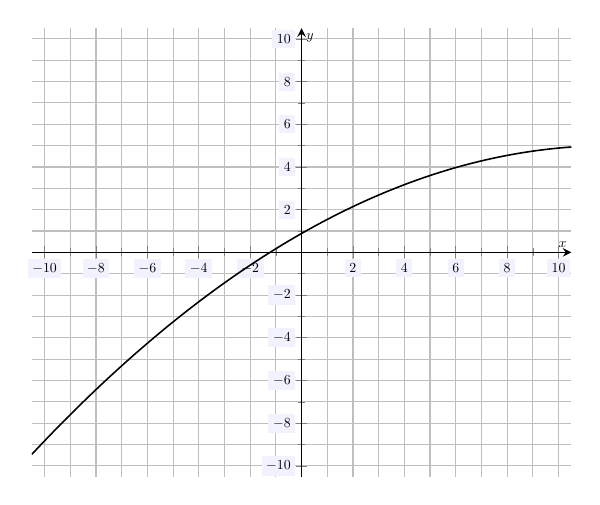
\begin{tikzpicture}[scale=1,every node/.style={scale=0.5}]
	\begin{axis}[
	grid=both,
	axis lines=middle,
	ticklabel style={fill=blue!5!white},
	xmin= -10.5, xmax=10.5,
	ymin= -10.5, ymax=10.5,
	xtick={-10,-8,-6,-4,-2,0,2,4,6,8,10},
	ytick={-10,-8,-6,-4,-2,0,2,4,6,8,10},
	minor tick = {-10,-9,...,10},
	xlabel=\(x\),ylabel=\(y\),
	]
	\addplot[line width= 0.02cm,samples=100,domain= -10.5:10.5] ({x},{5 - 1/35*(x - 12)^2});
	\end{axis}
	\end{tikzpicture}
	}
	\] 
This function is clearly everywhere increasing, so that $f'(x) > 0$. However, observe that the function is concave down, so that $f''(x) < 0$. The sign of $f'$ and $f''$ do indeed give you information about $f(x)$. However, the signs of $f$, $f'$, and $f''$ \textit{do not} need to be the same. \pvspace{1.3cm}











\end{document}